
\section{Introduction}

This chapter describes the practical implementation of the proposed solution.
It presents the dataset structure, the preprocessing workflow, the feature engineering strategy, the machine learning pipeline, and the design of the interactive Streamlit dashboard.

\section{Business Understanding}

The business objective of the project is to support a better understanding of housing market dynamics in the United States.
The analytical objective is to learn the relationship between macroeconomic variables and a housing-related target variable, then use that relationship to estimate future trends.

The practical outcome expected from the project is not only a predictive model, but also an application that allows users to inspect data and interpret results visually.

\section{Dataset Presentation}

The dataset used in this project contains a date column and several numerical indicators related to housing and macroeconomic conditions.
Although exact variable names may depend on the source file, the dataset generally includes a housing price metric together with economic features such as inflation, unemployment, and interest rates.

The first step was to inspect the structure of the data:
\begin{itemize}
\item identify the date column,
\item verify numerical columns,
\item detect missing values,
\item and evaluate duplicate observations.
\end{itemize}

\section{Data Preparation}

\subsection{Date Parsing}

Because the project includes a strong time-series component, parsing the date column correctly was essential.
The date variable was converted into a valid datetime format and the dataset was sorted chronologically.

\subsection{Numeric Conversion}

All features expected to be numerical were converted explicitly.
This step reduced the risk of hidden formatting issues and ensured that the models could process the variables correctly.

\subsection{Missing Values}

Missing values are common in real datasets.
Instead of removing every incomplete row, the project used imputation strategies in the machine learning pipeline.
Median imputation was selected because it is simple, robust, and appropriate for many economic indicators.

\subsection{Filtering and Data Quality Checks}

The dashboard also includes data quality indicators such as:
\begin{itemize}
\item number of rows,
\item number of columns,
\item total missing cells,
\item duplicate rows,
\item number of detected periods.
\end{itemize}

These checks provide immediate feedback to the user before advanced analysis begins.

\section{Feature Engineering}

Feature engineering improves the quality of the information provided to the models.
In this project, two forms of feature engineering were especially important.

\subsection{Administrative Period Labeling}

A categorical variable called \textit{administration} was derived from the date column.
This variable groups observations into periods such as:
\begin{itemize}
\item Pre-Trump,
\item Trump (2017--2020),
\item Biden (2021--2024),
\item Post-Biden.
\end{itemize}

This feature helps compare economic and housing behavior across political periods.

\subsection{Lag and Rolling Features}

For forecasting, lagged variables and rolling averages were created.
Examples include:
\begin{itemize}
\item target lag at 1, 3, 6, and 12 periods,
\item rolling means,
\item first differences,
\item lagged explanatory variables.
\end{itemize}

These engineered features make the forecasting stage more informative because they capture temporal dependence.

\section{Dashboard Architecture}

The dashboard was developed with Streamlit and divided into several tabs.
This structure improves navigation and keeps related analyses together.

The main tabs include:
\begin{enumerate}
\item Goal and interpretation,
\item Data quality,
\item Time series,
\item Correlations and scatter plots,
\item Charts,
\item Trump vs Biden comparison,
\item Machine Learning,
\item Forecast,
\item Export.
\end{enumerate}

\subsection{Overview and Interpretation}

The first tab introduces the project objective and highlights the most correlated variables with the selected target.
This gives the user an immediate analytical summary.

\subsection{Data Quality}

The second tab focuses on missing values and general dataset structure.
This is important because users should understand the limitations of the data before trusting any prediction.

\subsection{Time Series Analysis}

A dedicated time series tab allows the visualization of the selected metric through time.
Rolling means can be added to smooth the evolution and highlight long-term trends.

\subsection{Correlation and Scatter Analysis}

The dashboard includes a correlation matrix for all numerical features.
It also allows users to choose two variables and visualize their relationship in a scatter plot with a trend line.
This makes the investigation of pairwise relationships much more intuitive.

\subsection{Distribution and Comparative Charts}

Box plots and violin plots are used to compare distributions across administrations.
This is useful for seeing whether one period systematically differs from another.

\section{Machine Learning Pipeline}

The machine learning module is designed to let the user choose:
\begin{itemize}
\item the target variable,
\item the explanatory features,
\item the scaling method,
\item and the model type.
\end{itemize}

The main steps of the pipeline are:
\begin{enumerate}
\item median imputation,
\item optional scaling,
\item model fitting,
\item test set prediction,
\item metric computation.
\end{enumerate}

\subsection{Selected Models}

Two models were selected:
\begin{itemize}
\item Ridge Regression, as an interpretable regularized baseline,
\item Random Forest, as a flexible ensemble method with stronger capacity to capture non-linear relationships.
\end{itemize}

\subsection{Train/Test Split}

The dataset is divided into training and testing subsets.
A chronological split is used instead of a random split in order to preserve the time order of the observations.
This is more appropriate for economic and temporal data.

\subsection{Performance Metrics}

The model results are summarized using MAE, RMSE, and \(R^2\).
These three metrics provide complementary perspectives:
MAE measures average absolute error, RMSE gives greater importance to large errors, and \(R^2\) evaluates explained variance.

\section{Forecasting Logic}

The forecasting tab extends the analytical value of the project.
A future horizon can be selected, and the target variable is projected step by step.
At each step, lag features and rolling statistics are recalculated so that the model can generate the next value.

Although this forecasting logic remains relatively simple compared with specialized time-series models, it is pedagogically useful and integrates well into the dashboard.

\section{Deployment}

The final system was deployed as a Streamlit application.
This deployment choice is well suited to the project because it transforms code into a user-friendly interface with minimal overhead.
The application can be launched locally and adapted easily if new variables or visualizations are added later.

\section{Conclusion}

This chapter presented the design and implementation of the complete solution.
It described how the data was prepared, how features were engineered, how the machine learning pipeline was structured, and how the dashboard was organized.
The next chapter presents the obtained results and discusses their interpretation.

\section{Application Architecture}

The application is implemented as a Streamlit dashboard that acts as the main entry point of the project. The code is organized around helper functions for data preparation, visualization, modeling, evaluation, reporting, and interface rendering. This architecture makes the application easier to maintain than a single block of procedural code.

\begin{figure}[H]
\centering
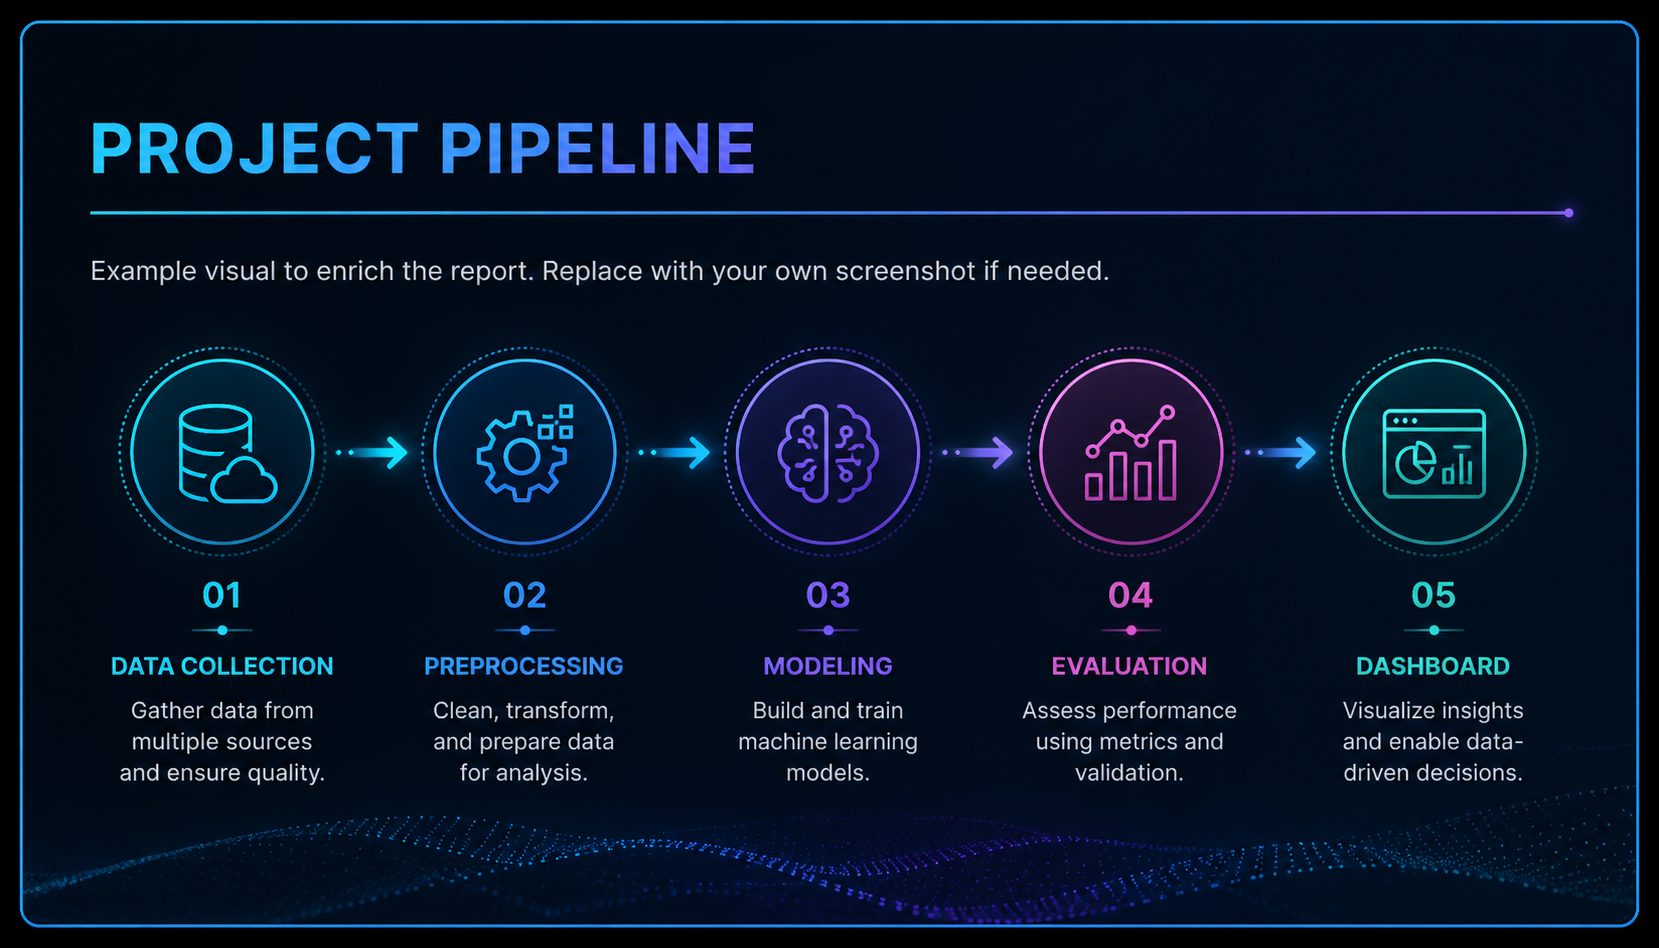
\includegraphics[width=0.95\textwidth]{project_pipeline (2).png}
\caption{End-to-end project pipeline from data loading to interpretation and deployment.}
\label{fig:project_pipeline}
\end{figure}

\subsection{Navigation Structure}

The dashboard navigation is organized to guide the user from general understanding to technical analysis and business interpretation. It contains pages for goal interpretation, data quality, time series, correlations, charts, administration comparison, machine learning, forecasting, export, and analytical pages such as:
\begin{itemize}
\item Overview,
\item Explore,
\item Data Quality,
\item ML Lab,
\item Evaluation,
\item Unsupervised Lab,
\item Reinforcement Lab,
\item Forecast,
\item OLAP and Export,
\item Scenario Simulator,
\item Paper Review,
\item Production Readiness,
\item Experiment Tracker,
\item Model Registry,
\item Data Pipeline,
\item Business Impact.
\end{itemize}

This expanded structure allows the project to cover the complete lifecycle of a data science product.

\section{Data Cleaning Module}

The application includes a documented data cleaning report. The objective is to show not only that the data was cleaned, but also what exactly was checked. The cleaning report includes column-name cleanup, date parsing, numeric conversion, missing-value checks, duplicate-row checks, period feature creation, and row preservation.

\begin{longtable}{p{4cm}p{5cm}p{5cm}}
\toprule
\textbf{Cleaning step} & \textbf{Purpose} & \textbf{Project value} \\
\midrule
Column-name cleanup & Remove leading and trailing spaces & Avoid hidden errors in feature selection. \\
Date parsing & Convert date column into datetime format & Enable chronological sorting and forecasting. \\
Numeric conversion & Convert numeric-looking text into numbers & Make features usable by models. \\
Missing-value check & Count missing cells before and after cleaning & Document data quality. \\
Duplicate-row check & Detect repeated observations & Prevent biased summaries. \\
Period feature creation & Add administration labels & Enable political-period comparison. \\
Row preservation & Verify that cleaning did not remove data unintentionally & Improve reproducibility. \\
\bottomrule
\caption{Data cleaning report logic.}
\end{longtable}

\section{Supervised Learning Module}

The supervised learning module includes a model laboratory. The application supports regression and classification modes and allows the user to compare several algorithms.

\subsection{Regression Models}

The regression models include Ridge Regression, Random Forest Regressor, Linear Regression, Support Vector Regressor, Gradient Boosting Regressor, Decision Tree Regressor, K-Nearest Neighbors Regressor, and Neural Network Regressor.

\subsection{Classification Models}

For classification, the numerical target can be transformed into categories such as low, medium, and high. The classification models include Random Forest Classifier, Logistic Regression, Decision Tree Classifier, K-Nearest Neighbors Classifier, and Neural Network Classifier.

\subsection{Pipeline Design}

The supervised learning pipeline follows this sequence:
\begin{enumerate}
\item Select target and features.
\item Remove rows with missing target values.
\item Split the dataset chronologically into training and testing subsets.
\item Impute missing feature values using the median.
\item Apply optional scaling using StandardScaler or MinMaxScaler.
\item Train the selected model.
\item Predict the test set.
\item Evaluate performance.
\item Display metrics and visual comparison.
\end{enumerate}

\section{Model Evaluation Module}

The evaluation page compares several models under the same conditions. This is important because a single model score is not enough to justify a modeling decision. The dashboard calculates regression metrics such as MAE, RMSE, and R squared, and classification metrics such as accuracy, precision, recall, F1-score, and ROC AUC when available.

\begin{longtable}{p{3cm}p{5cm}p{6cm}}
\toprule
\textbf{Metric} & \textbf{Used for} & \textbf{Interpretation} \\
\midrule
MAE & Regression & Average absolute prediction error. Lower is better. \\
RMSE & Regression & Penalizes large errors more strongly. Lower is better. \\
R squared & Regression & Share of variance explained by the model. Higher is better. \\
Accuracy & Classification & Share of correct predictions. Higher is better. \\
Precision & Classification & Reliability of positive predictions. Higher is better. \\
Recall & Classification & Ability to detect true positive cases. Higher is better. \\
F1-score & Classification & Balance between precision and recall. Higher is better. \\
ROC AUC & Classification & Ranking quality across classes. Higher is better. \\
\bottomrule
\caption{Evaluation metrics used in the dashboard.}
\end{longtable}

\section{Unsupervised Learning Module}

The unsupervised learning page adds exploratory intelligence beyond the supervised target. Its objective is to discover structures that may not be visible in standard charts.

\subsection{K-Means Implementation}

The user selects numerical features and a number of clusters. The features are scaled, the K-Means algorithm is fitted, and the resulting cluster labels are visualized. This helps identify groups of months or observations with similar economic profiles.

\subsection{DBSCAN Implementation}

DBSCAN is used to identify dense regions and outliers. It is particularly useful for detecting unusual market periods. The user can adjust parameters such as neighborhood size and minimum samples.

\subsection{PCA Visualization}

PCA reduces the selected features to principal components. The first two components can be plotted to visualize the structure of the dataset. PCA also helps understand whether the dataset contains strong dominant dimensions.

\subsection{Anomaly Detection}

Isolation Forest identifies observations that are statistically unusual compared with the majority of the data. In housing analysis, such observations may correspond to crisis periods, high-rate shocks, or abnormal combinations of macroeconomic indicators.

\section{Reinforcement Learning Module}

The reinforcement-learning page is an educational module. It illustrates how a decision-making agent can learn from rewards. The module is not intended to provide investment recommendations; instead, it demonstrates the concepts of state, action, reward, and policy.

A simplified housing-market state can be based on indicators such as price trend, interest-rate pressure, and unemployment behavior. Possible actions can include conservative decision labels such as wait, monitor, or act. The reward function evaluates whether the chosen action was suitable under the simulated environment.

\section{OLAP and Export Module}

The OLAP module allows the user to build summarized views of the dataset. The most important OLAP outputs are grouped tables and pivot-style summaries.

Examples of OLAP questions include:
\begin{itemize}
\item What is the average housing price index by administration period?
\item Which period has the highest mean mortgage rate?
\item How do unemployment and inflation compare across periods?
\item Which indicators changed the most between Trump and Biden periods?
\end{itemize}

The export functionality allows users to download relevant tables. This is useful for reports, presentations, and further analysis.

\section{Scenario Simulator}

The scenario simulator is designed for what-if analysis. It allows the user to modify feature values and observe the expected effect on the model output. This helps transform the dashboard from a passive reporting tool into an interactive decision-support system.

Scenario simulation is especially useful in economic analysis because users often ask questions such as:
\begin{itemize}
\item What happens if mortgage rates increase?
\item What happens if unemployment rises?
\item How sensitive is the target to inflation?
\item Which feature change produces the strongest predicted movement?
\end{itemize}

\section{AI Chatbot and Prompt Chatbot Implementation}

The code contains optional OpenAI integration. The application is designed to run even when the OpenAI package or API key is not available. This makes the system robust: users can still use the dashboard without chatbot access, while users with a valid configuration can activate AI assistance.

The chatbot supports natural language interaction. The prompt chatbot complements it by guiding users toward structured analytical questions. This is useful for non-technical users who need explanations of data science outputs.

\section{Paper Review and Real-Market Comparison Module}

The paper review page connects the application results with economic theory and real-world housing-market periods. Instead of presenting machine learning as a black-box exercise, the project compares the dataset behavior with expectations from housing economics.

The module includes theory checks based on expected correlation signs, real-life period comparison, final conclusion generation, and interpretation of why some relationships support or challenge theory.

\section{Production Readiness Module}

The production-readiness page introduces practical checks that would be necessary before deploying a data science product in a professional environment. These checks include dataset validity, missingness, duplicates, date-column availability, target availability, and model governance notes.

This module is important because it shows that the project is not only an academic experiment. It considers how the system could be maintained and monitored in real use.

\section{Experiment Tracker and Model Registry}

The experiment tracker records model runs and their metrics. This allows users to compare experiments over time. The model registry identifies the best candidate model and documents whether it can be promoted as a champion model.

In professional data science, this step is essential because models must be traceable. If a model is used later, the team must know how it was trained, which data was used, and what performance it achieved.

\section{Deployment Logic}

The application is deployed with Streamlit. Streamlit was selected because it allows fast transformation of Python analysis into an interactive web application. The interface includes custom styling with custom styling, sidebar navigation, searchable dashboard destinations, dark/light mode logic, and user-friendly cards.

The deployment workflow is:
\begin{enumerate}
\item Install Python dependencies.
\item Place the dataset in the expected data folder or upload it through the interface.
\item Launch the app using Streamlit.
\item Use the dashboard pages to explore, model, evaluate, export, and interpret results.
\end{enumerate}

\section{Code Organization}

Although the current Streamlit file is the main entry point, the code is written with reusable helper functions. In a future professional implementation, these helpers could be moved into a package such as \texttt{src/us\_housing}. This would separate data preparation, modeling, UI rendering, and reporting logic.

\begin{table}[H]
\centering
\begin{tabularx}{\textwidth}{lX}
\toprule
\textbf{Code component} & \textbf{Role} \\
\midrule
Data helpers & Detect dates, clean data, build reports, calculate correlations. \\
UI helpers & Render metric cards, learning cards, search results, and dashboard layout. \\
Model helpers & Build pipelines, train models, compare algorithms, calculate metrics. \\
Interpretation helpers & Summarize correlations, theory checks, real-life period comparison. \\
Governance helpers & Build data dictionaries, validation reports, executive reports, and model registry outputs. \\
\bottomrule
\end{tabularx}
\caption{Code organization by functional role.}
\end{table}

\section{Conclusion of the Implementation}

The implementation presents a complete housing intelligence platform. It now covers the main pillars of a modern data science product: data preparation, exploratory analysis, supervised learning, unsupervised learning, forecasting, OLAP, chatbot interaction, paper comparison, governance, and deployment.
